% !TeX root = ../main.tex
\section{Reinitialize Bad Starts Study}
\label{sec:relu1-reinit}

\subsection*{Study Motivation}

The baseline analysis identified dead data as the primary failure mechanism limiting success to 48\%. When XOR points have negative pre-activation across both ReLU units, they cannot contribute gradient signals for error correction, creating learning asymmetries that prevent successful mirror symmetry discovery. Statistical analysis revealed that 39 of 50 runs began with dead inputs, with success rates dropping dramatically from 82\% for clean-start runs to 38\% for runs with initial dead data.

This failure mode suggests a direct intervention strategy: eliminate dead data at initialization rather than attempting to recover from it during training. The approach involves re-initializing networks using standard Kaiming principles until all four XOR points produce positive pre-activation in each ReLU unit, ensuring that gradient flow is preserved from the outset of training.

The core research question is empirical: how much does eliminating dead data at initialization improve success rates? If dead data represents the primary bottleneck, this simple screening approach should provide substantial performance gains with minimal implementation overhead. Based on initial results, we also explore whether requiring activation margins above zero (>0.3) provides additional benefits beyond basic dead data elimination.

This initialization-based intervention offers several advantages: it preserves established Kaiming initialization principles while addressing the identified failure mode, requires no architectural modifications or training procedure changes, and provides a direct test of the dead data hypothesis through targeted elimination of the problematic initial conditions.

% ------------------------------------------------------------------

\subsection*{Study Design}

\paragraph{Experimental Variants}
The study tests two reinitialization strategies against the baseline Kaiming initialization that achieved 48\% success. The basic reinitialization variant re-samples initialization until all four XOR points produce positive pre-activation in at least one ReLU unit, eliminating dead data while maintaining minimal constraints. The margin reinitialization variant tightens this criterion, requiring all XOR points to achieve pre-activation values greater than 0.3 in at least one ReLU unit, providing additional separation from the activation threshold.

\paragraph{Reinitialization Protocol}
Both variants employ iterative sampling using standard Kaiming normal initialization with weights drawn from $\mathcal{N}(0, \sigma)$ and bias initialized to zero. For each initialization attempt, pre-activation values are computed for all four XOR points across both ReLU units. The basic variant accepts any configuration where $\max_k f_k(x_i) > 0$ for every input $x_i$, while the margin variant requires $\max_k f_k(x_i) > 0.3$. If the criteria are not met, the network is re-initialized up to a maximum of 100 attempts before proceeding with the best available configuration.

\paragraph{Training Protocol}
All variants maintain identical training procedures to isolate the impact of initialization improvements. The same two-ReLU architecture (Linear(2→2) → ReLU → Sum) is used with consistent Adam optimizer parameters and early stopping criteria from the baseline study. Statistical analysis employs 50 independent runs for the basic reinitialization variant and 500 runs for the margin variant to capture the improved reliability with sufficient precision.

\paragraph{Analysis Framework}
The experimental design enables direct assessment of dead data elimination effectiveness through success rate comparison, convergence timing analysis, and geometric characterization. Success metrics quantify the performance improvement over the 48\% baseline, while convergence analysis reveals any training efficiency changes from improved initialization. Geometric analysis examines whether eliminating dead data promotes the theoretically predicted mirror-symmetric patterns through distance clustering, weight space analysis, and symmetry detection. Failure mode analysis characterizes any residual failures to identify remaining bottlenecks beyond dead data elimination.

% ------------------------------------------------------------------

\subsection*{Success Metrics}

\begin{table}[ht]
\centering
\caption{Classification accuracy comparison across reinitialization strategies.}
\label{tab:relu1-reinit-success}
\begin{tabular}{lccc}
\toprule
Variant & Success Rate & Performance vs Baseline & Runs \\
\midrule
ReLU (Baseline) & 24/50 (48\%) & -- & 50 \\
Reinit (basic) & 46/50 (92\%) & +92\% relative & 50 \\
Reinit + margin 0.3 & 496/500 (99.2\%) & +107\% relative & 500 \\
\bottomrule
\end{tabular}
\end{table}

Dead data elimination through reinitialization provides dramatic performance improvements, with basic reinitialization nearly doubling the success rate from 48\% to 92\%. Both reinitialization variants achieve perfect dead data elimination, with all runs showing "no dead inputs" throughout training, confirming that the intervention successfully addresses the primary failure mechanism identified in the baseline analysis.

However, the persistence of failures despite clean initialization reveals a secondary failure mode. Analysis of the 4 failed runs from basic reinitialization showed hyperplanes positioned extremely close to individual data points. These proximity-based configurations create geometric vulnerabilities where hyperplanes can easily enter dead states during training despite starting with positive activations. This observation motivated the margin requirement intervention.

\begin{table}[ht]
\centering
\caption{Failure analysis across reinitialization variants.}
\label{tab:relu1-reinit-failures}
\begin{tabular}{lcccc}
\toprule
Variant & Total Failures & Failure Rate & 75\% Accuracy & Failure Pattern \\
\midrule
ReLU (Baseline) & 26/50 & 52\% & 26 & Mixed (dead data + geometric) \\
Reinit (basic) & 4/50 & 8\% & 4 & Geometric (proximity) \\
Reinit + margin 0.3 & 4/500 & 0.8\% & 4 & Geometric (proximity) \\
\bottomrule
\end{tabular}
\end{table}

The margin requirement demonstrates substantial effectiveness, reducing failures from 8\% to 0.8\%—a ten-fold improvement. The 0.3 activation threshold prevents most proximity-based failures by ensuring hyperplanes begin with sufficient separation from all data points. However, the persistence of 4 failures among 500 runs indicates that the margin provides substantial but not complete protection against geometric vulnerabilities.

All remaining failures across both reinitialization variants reach exactly 75\% accuracy, reflecting XOR's discrete accuracy constraints and confirming a consistent geometric failure mode distinct from the gradient-based dead data problem. The progressive improvement from baseline (52\% failure) through basic reinitialization (8\% failure) to margin requirements (0.8\% failure) demonstrates that reliability can be systematically enhanced through targeted geometric interventions.

The results establish that dead data elimination is necessary but not sufficient for reliable learning. While the primary bottleneck involves gradient flow preservation, secondary geometric vulnerabilities require additional safeguards to achieve near-perfect success rates.

% ------------------------------------------------------------------

\subsection*{Learning Dynamics}

\begin{table}[ht]
\centering
\caption{Convergence timing for successful runs (100\% accuracy only, epochs to MSE < $10^{-7}$).}
\label{tab:relu1-reinit-timing}
\begin{tabular}{lcccccc}
\toprule
\multirow{2}{*}{Variant} &
\multicolumn{5}{c}{Epoch percentile} & \multirow{2}{*}{Count} \\
\cmidrule(lr){2-6}
& 0\,\% & 25\,\% & 50\,\% & 75\,\% & 100\,\% & \\
\midrule
ReLU (Baseline) & 53 & 126 & 190 & 251 & 336 & 24/50 \\
Reinit (basic) & 37 & 95 & 151 & 255 & 343 & 46/50 \\
Reinit + margin 0.3 & 42 & 129 & 181 & 252 & 457 & 496/500 \\
\bottomrule
\end{tabular}
\end{table}

Dead data elimination through reinitialization produces modest improvements in training efficiency for successful runs. Basic reinitialization reduces median convergence time from 190 to 151 epochs, while margin reinitialization achieves median convergence at 181 epochs. The timing improvements reflect the optimization benefits of starting with active gradient signals from all data points rather than having to recover from dead configurations during training.

```latex
The convergence timing patterns remain remarkably consistent across reinitialization variants, with successful runs following similar optimization trajectories regardless of initialization strategy. This consistency suggests that once learning begins effectively, the underlying optimization dynamics are largely independent of the specific initialization approach. The slightly longer convergence times for margin reinitialization (181 vs 151 epochs median) likely reflect the more stringent initialization requirements, which may occasionally require starting configurations that are further from optimal mirror-symmetric patterns.
```

The training efficiency gains, while modest in absolute terms, become significant when combined with the dramatic success rate improvements. Basic reinitialization achieves both higher reliability (92\% vs 48\%) and faster convergence for successful runs, while margin requirements maintain reasonable training speeds despite the additional geometric constraints. These results demonstrate that addressing initialization quality provides benefits for both success rates and optimization efficiency.

% ------------------------------------------------------------------

\subsection*{Geometric Analysis}

The geometric analysis reveals how eliminating problematic initialization conditions promotes the discovery of theoretically predicted mirror-symmetric patterns. Dead data elimination and margin requirements systematically improve solution quality and geometric consistency across multiple measures.

\begin{table}[ht]
\centering
\caption{Distance pattern evolution across reinitialization strategies.}
\label{tab:relu1-reinit-distance}
\begin{tabular}{lcccc}
\toprule
Variant & Class 0 Distance & Class 1 Distance & Distance Clusters & Hyperplanes \\
\midrule
ReLU (Baseline) & $0.32 \pm 0.21$ & $1.37 \pm 0.05$ & 1 & 48 \\
Reinit (basic) & $0.32 \pm 0.19$ & $1.37 \pm 0.04$ & 1 & 92 \\
Reinit + margin 0.3 & $0.36 \pm 0.17$ & $1.36 \pm 0.05$ & 1 & 992 \\
\bottomrule
\end{tabular}
\end{table}

Distance pattern analysis confirms that all reinitialization variants maintain the core prototype surface relationship, with False class points positioned near learned hyperplanes and True class points at the expected distance around $\sqrt{2}$. The margin requirement produces the predicted geometric effect: Class 0 distances increase from $0.32 \pm 0.19$ to $0.36 \pm 0.17$, reflecting the enforced 0.3 activation threshold that prevents hyperplanes from starting too close to data points. The reduced variance in margin reinitialization suggests more consistent geometric positioning.

\begin{table}[ht]
\centering
\caption{Weight clustering and mirror symmetry across reinitialization strategies.}
\label{tab:relu1-reinit-symmetry}
\begin{tabular}{lcccc}
\toprule
Variant & Mirror Pairs & Perfect Mirrors & Weight Clusters & Noise Points \\
\midrule
ReLU (Baseline) & 16/50 (32\%) & 3 & 9 & 10 \\
Reinit (basic) & 39/50 (78\%) & 13 & 7 & 8 \\
Reinit + margin 0.3 & 441/500 (88\%) & 79 & 5 & 6 \\
\bottomrule
\end{tabular}
\end{table}

The weight space analysis demonstrates progressive geometric improvement through each intervention level. Dead data elimination more than doubles mirror pair detection from 32\% to 78\%, while margin requirements further increase mirror symmetry to 88\%. Perfect mirror symmetry detection shows even more dramatic improvement, increasing from 3 instances in the baseline to 79 in the margin variant. This progression validates the theoretical prediction that clean initialization enables networks to discover the optimal $w^{(1)} = -w^{(0)}$ relationship.

Weight clustering analysis reveals systematic solution consolidation as initialization quality improves. The baseline's 9 clusters with 10 noise points reduces to 7 clusters with 8 noise points for basic reinitialization, and further consolidates to 5 clusters with 6 noise points for margin requirements. This reduction in solution diversity indicates that eliminating problematic initialization conditions channels networks toward a smaller set of high-quality patterns, with the margin variant showing two dominant mirror-symmetric clusters covering the vast majority of successful runs.

The geometric improvements demonstrate that learning benefits significantly from proper initialization conditions. Clean starts not only improve success rates but also promote discovery of the theoretically optimal mirror-symmetric solutions, confirming that the geometric predictions of prototype surface theory emerge more reliably when optimization begins from well-conditioned configurations.

% ------------------------------------------------------------------

\subsection*{Aim}
The baseline showed that plain Kaiming weights often leave at least one
XOR point \emph{inactive} for every neuron.  
Here we test a simple remedy: \textbf{re-initialise the network up to 100 times 
until all four inputs produce a positive pre-activation in \emph{each} ReLU}, 
using Kaiming-normal initialization with weights \(\sim \mathcal{N}(0, \sigma)\) and bias \(0\), as in Section~\ref{sec:relu1-kaiming}.
The reinitialization ensure that the network begins training without any dead data.
A second variant tightens the criterion by requiring a \emph{margin}
of $0.3$ in activation space.

\begin{description}[leftmargin=2em,style=sameline]
  \item[\texttt{relu1\_reinit}]   stop once \(\max_k f_k(x_i) > 0\) for every \(x_i\);
  \item[\texttt{relu1\_reinit\_margin}] stop once each \(x_i\) satisfies
        \(\max_k f_k(x_i) > 0.3\).
\end{description}
Both use the same optimiser and early-stop rules as previous sections.

% ------------------------------------------------------------------
\subsection*{Classification Accuracy}

\begin{table}[ht]
\centering
\caption{Final accuracy across runs.}
\label{tab:relu1-reinit-accuracy}
\begin{tabular}{lccccc}
\toprule
Variant & 0\,\% & 25\,\% & 50\,\% & 75\,\% & 100\,\% \\
\midrule
Baseline (ReLU)       & 0 & 0 & 0 & 26 & 24 \\
Reinit (no margin)    & 0 & 0 & 0 & 5  & 45 \\
Reinit + margin 0.3   & 0 & 0 & 0 & 4  & 496/500 \\
\bottomrule
\end{tabular}
\end{table}

\paragraph{Headline}
A single pass of dead-data re-init lifts success from
$48\,\%\!\to\!90\,\%$;
adding the $0.3$ margin pushes reliability to \(\approx99\,\%\).

% ------------------------------------------------------------------
\subsection*{Convergence Timing}

\begin{table}[ht]
\centering
\caption{Epochs to early-stop (successful runs only).}
\label{tab:relu1-reinit-epochs}
\begin{tabular}{lccccc}
\toprule
Variant & 0\,\% & 25\,\% & 50\,\% & 75\,\% & 100\,\% \\
\midrule
Reinit            & 26 & 119 & 168 & 233 & 336 \\
Reinit + margin   & 44 & 132 & 190 & 255 & 448 \\
\bottomrule
\end{tabular}
\end{table}

Median training time increases modestly under the margin rule because
the initial sampling occasionally needs several tries.

% ------------------------------------------------------------------
\subsection*{Hyperplane Geometry}

\begin{description}[leftmargin=2em]
  \item[Distance clusters] Both variants collapse to a \emph{single}
        distance pattern, as in the baseline, but the class-0 distances
        shift from \(0.29\pm0.20\) (no margin) to
        \(0.36\pm0.17\) with margin, reflecting the enforced offset.%
        
  \item[Weight clusters] Dead-data re-init reduces the number of weight
        clusters from nine (baseline) to seven; the margin variant
        compresses them to six with a dominant pair of mirror-centroids
        covering $>95\,\%$ of runs.%
  \item[Mirror symmetry] Mirror pairs rise from
        $37/50$ (74\,\%) to $442/500$ (88\,\%) and the count of
        \emph{perfect} mirrors almost doubles
        (11 → 94).%
\end{description}

\subsection*{Emergent Failure Modes}
A second failure pattern surfaces even after dead-data screening:
in rare cases hyperplanes fall into a local basin that is almost
\emph{perpendicular} to any solution-bearing orientation (example shown in Fig.\,\ref{fig:reinit-bad}).
These runs account for the residual $75\,\%$ accuracies in both tables. 
We notice that this hyperplane is also dead and does not intersect the data space.
It is not clear how the initial state relates to this basin.

\begin{figure}[ht]
  \centering
  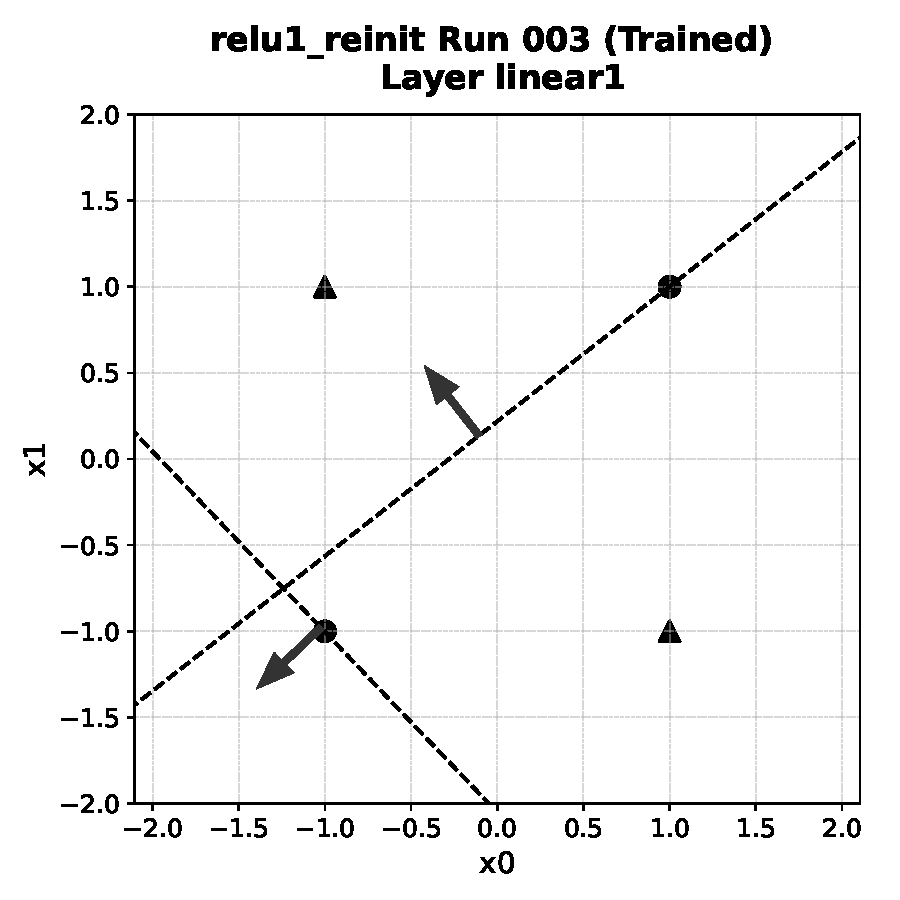
\includegraphics[width=0.38\textwidth]{relu1/figs/reinit_bad_example.pdf}
  \caption{Illustration of the "perpendicular" failure: the left dashed
           line rotates perpendicular to the optimal position.}
  \label{fig:reinit-bad}
\end{figure}

% ------------------------------------------------------------------
\paragraph{Study Discussion}
\begin{itemize}
  \item Screening out dead inputs at \emph{initialisation} is a
        lightweight, one-shot fix that triples the reliability of the
        two-ReLU model.
  \item Enforcing a small positive margin further reduces variance at the
        cost of extra sampling time, moving success toward certainty.
  \item Prototype-surface geometry tightens: mirror solutions dominate
        and distance clusters homogenise, reinforcing the theory's
        prediction that symmetry emerges once every input is alive.
  \item The remaining errors stem from a distinct "dying-ReLU" 
        trap, which motivates the runtime monitors discussed next.
\end{itemize}

\hrulefill
